\section{The Testbench Architecture}\label{sec:testbench-architecture}

\begin{figure}
    \centering
    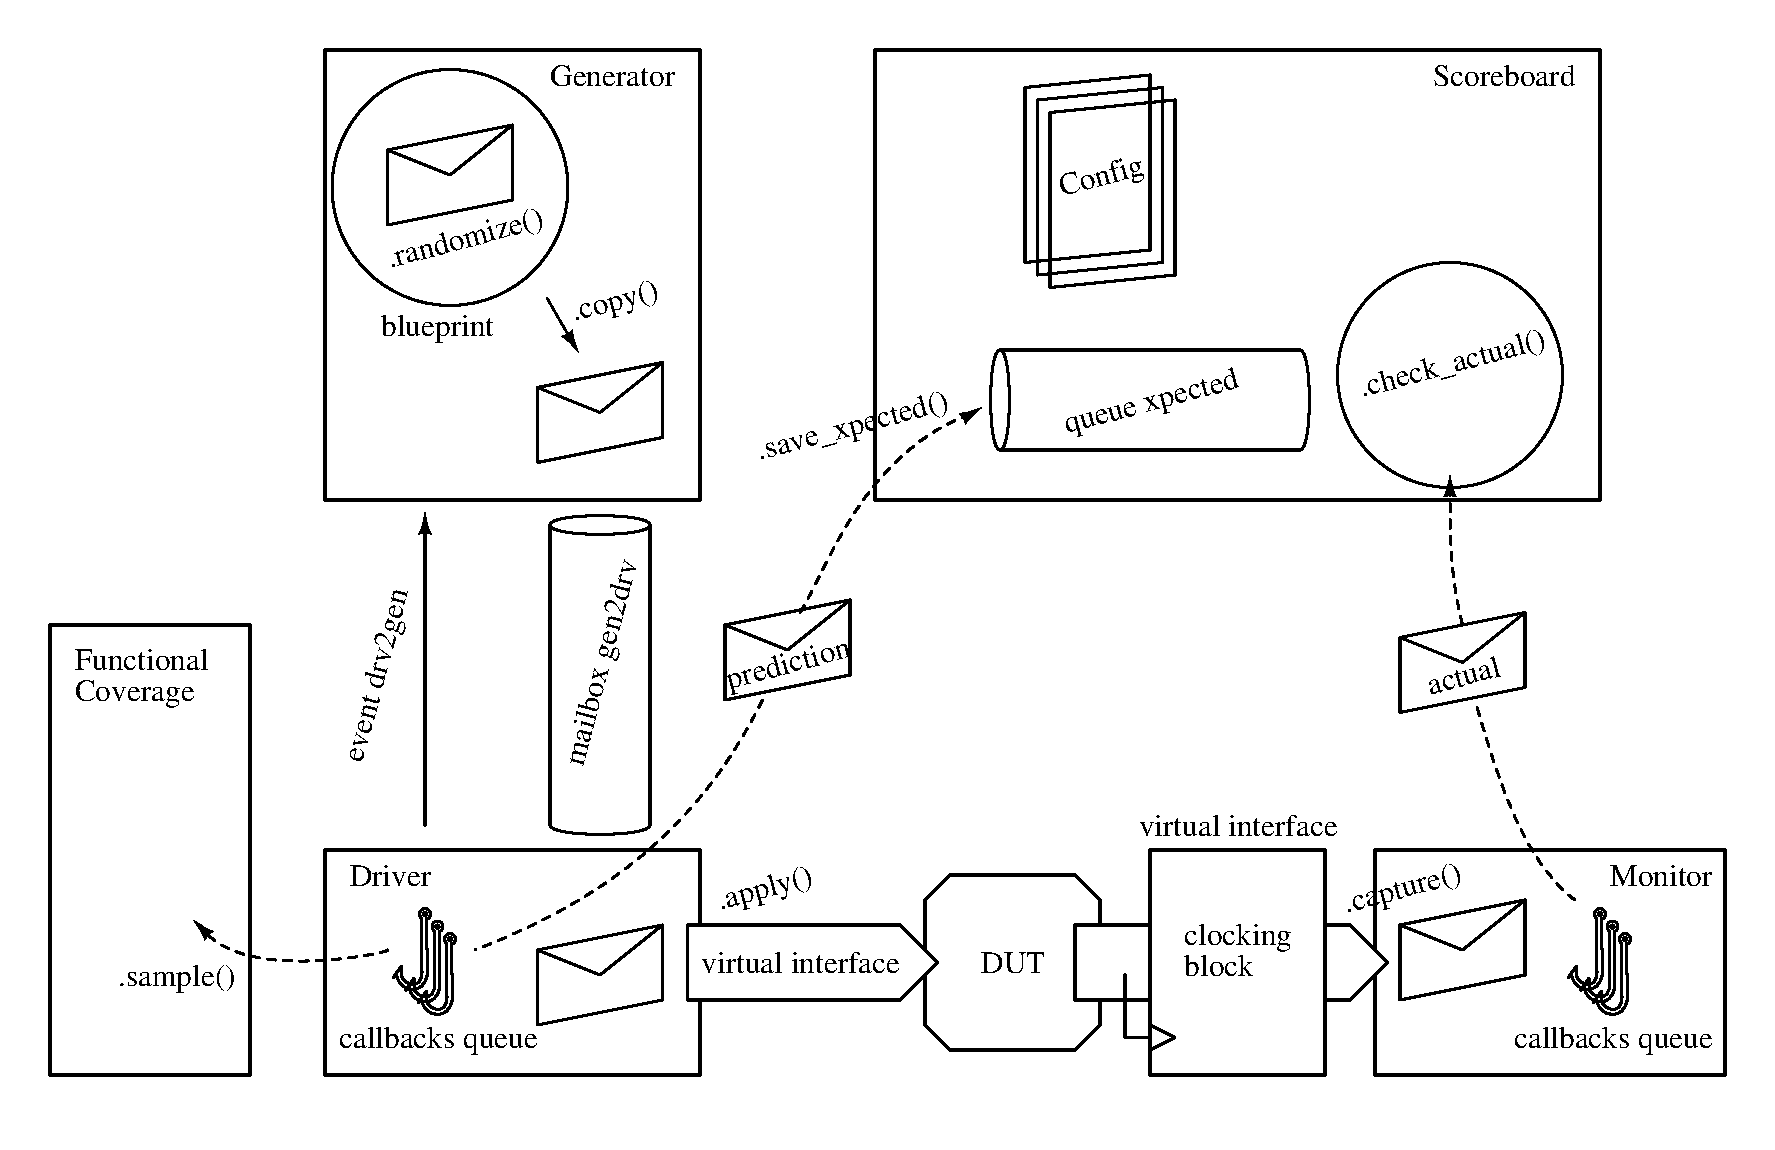
\includegraphics[width=\textwidth]{fig/bench.eps}
    \caption{Conceptual representation of the layered testbench environment and its interface to the \ac{dut}. The dashed arrows highlight the callback calls; the letter envelopes mark the path followed by transactions around the testbench.}
    \label{fig:bench}
\end{figure}

The architecture of the developed testbenches is conceptually represented in~\cref{fig:bench}. The idea I had in mind sprouted from my previous experiences with \CC and a more recent exposure to SystemC. The goal was to exploit both \ac{oop} and generic programming capabilities of \sv to build a reusable, templated testbench framework that could later be specialized for specific \ac{dut}s. In the quest for already published works on the topic, I found~\cite{spear:svfe} as a concrete example of what the final testbench environment could look like. 

A significant novelty compared to general-purpose object-oriented languages is that data hiding is not stressed by the language; for instance, in \CC the default access to class members is private. I chose to stick with this default as a way to simplify code development.

\subsection{The Core Components}

\begin{listing}
\begin{minted}[bgcolor=mintedbackground, fontsize=\scriptsize]{systemverilog}
class Generator
  #(type T = BaseTransaction);

  T blueprint;
  ...

  task run();
    T tr; // host the cloned blueprint

    repeat (n_tr) begin
      `SV_RAND_CHECK(blueprint.randomize()); // so to keep randomization history
      $cast(tr, blueprint.copy()); // then, copy

      tr.display($sformatf("@%0t: Generator: ", $time));

      gen2drv.put(tr); // send the transaction
      @drv2gen;        // the driver has finished with it
    end;

  endtask : run
endclass
\end{minted}
\caption{The snippet highlights how type template parameters can improve code reusability, greatly reducing development time. \svinline{$cast()} here is an example of dynamic downcasting: \svinline{copy()} returns a base class handle that gets cast to point to the child class \svinline{T}.}
\label{list:gen}
\end{listing}

\noindent The reusable core components are:
\begin{description}
    \item[\svinline{virtual class BaseTransaction}] Information gets passed around the testbench encapsulated in transaction objects. This abstract class is devised to be used as a base for inheritance and defines some fundamental methods to be used by other core components. For instance, \svinline{copy()} shown in~\cref{fig:bench}, which gets called inside the \svinline{Generator} class to make copies of the blueprint transaction object.
    
    \item[\svinline{class Generator}] The generator is responsible for creating random transactions and dispatching them to the driver through a mailbox, a communication channel that behaves like a FIFO. 
    
    The \emph{blueprint} pattern is a convenient \ac{oop} technique here employed so that by changing this reference object it's possible to control the stream of generated transactions: the blueprint is repeatedly randomized, cloned and the clone gets sent through the mailbox. A significant reason for choosing to use this pattern is that, given that it's the blueprint object that gets randomized instead of the clone, the random-cyclic behavior of any \svinline{randc} member of the transaction class is respected.

    The class is templated with the transaction type for flexibility, as shown in~\cref{list:gen}.
    
    \item[\svinline{class Callback}] Callbacks are a powerful mechanism in the testbench architecture, not only when it comes to reusing code for later projects, but also for developing a single verification environment that can be shared by all tests. To achieve that, there are "hooks" where tests or other environment modules can dynamically inject new code to execute.
    
    \item[\svinline{class Config}] The config class serves as the central configuration descriptor for the testbench. In this case, for simplicity, I hardcoded the parsing of the command-line argument \mintinline{text}{+n_packets}, which allows changing the number of packets to generate to a value other than the default 10.
    
    \item[\svinline{class Scoreboard}] The scoreboard acts as the central hub for collecting and verifying the expected and actual responses from the \ac{dut}. It connects to the driver and monitor modules via callbacks:
    \begin{itemize}
        \item the driver receives from the generator the stream of transactions to be applied to the \ac{dut}. After having applied each of them, it shall execute a hook to fill the transaction with the expected \ac{dut}'s response and save it in the scoreboard.
        \item every time the monitor captures a response from the \ac{dut}, it shall execute a hook to make the scoreboard compare it with the expected one.
    \end{itemize}
    \item[\svinline{virtual class BaseEnvironment}] The environment is an abstract class that encapsulates all the blocks of the layered testbench and is devised as a base for inheritance. It simulates everything that is not inside the DUT, making it possible to run a certain testbench program via: 
    \begin{itemize}
        \item \svinline{build()}, a method left to be implemented by child classes. It shall build the environment, which encompasses the allocation of the transactors and of the callbacks and their registration with both the scoreboard and the coverage class.
        \item \svinline{run()}. The generator, the driver and the monitor classes are run in their own threads. A timeout block prevents the simulation to hang in case of errors.
        \item \svinline{wrap_up()}, which prints a statistic of the current run, reporting the number of errors and the total functional coverage.
    \end{itemize}
\end{description}

\subsection{\acs{dut} - \acl{alu}}\label{subsec:dut_alu}

\begin{listing}
\begin{minted}[bgcolor=mintedbackground, fontsize=\scriptsize]{vhdl}
package type_alu is
  type type_op is (add, sub, mult, bitand, bitor, bitxor, funclsl, funclsr, funcrl, funcrr);
end package;

entity alu is
  generic (n : integer);
  port ( 
    func:         in  type_op;
    data1, data2: in  std_logic_vector(n-1 downto 0);
    outalu:       out std_logic_vector(n-1 downto 0)
  );
end entity;
\end{minted}
\caption{\vhdl interface of the \ac{alu} under test. \mintinline{vhdl}{type_op} is an enumerated type defined in a \vhdl package, imported into \sv namespaces when necessary.}
\label{list:dut_alu}
\end{listing}

\noindent The \ac{alu} is designed to meet the following specifications:
\begin{itemize}
    \item support for different word sizes
    \item support for various combinational operations:
    \begin{itemize}
        \item \emph{addition}, \emph{subtraction} on full-width operands
        \item \emph{multiplication} on half-width operands
        \item \emph{and}, \emph{or}, \emph{xor} on full-width operands
        \item \emph{left/right shift} and \emph{rotate} on a number of positions specified by the second operand.
    \end{itemize}
\end{itemize}

\subsubsection{The Testbench Refinement}

\begin{listing}
\begin{minted}[bgcolor=mintedbackground, fontsize=\scriptsize]{systemverilog}
constraint ab_dist_c {
    a dist {
      0                         := 10,
      [1:(64'd1<<DATA_WIDTH)-2] :/ 1,
      (64'd1<<(DATA_WIDTH-1))-1 := 10,
      (64'd1<<DATA_WIDTH)-1     := 10
      };
    b dist {
      0                         := 10,
      [1:(64'd1<<DATA_WIDTH)-2] :/ 1,
      (64'd1<<(DATA_WIDTH-1))-1 := 10,
      (64'd1<<DATA_WIDTH)-1     := 10
    };
  };
\end{minted}
\caption{Weighted distribution constraint for the \ac{alu} input operands.}
\label{list:alu_ab_dist}
\end{listing}

\begin{listing}
\begin{minted}[bgcolor=mintedbackground, fontsize=\scriptsize]{systemverilog}
class AluDriver;
  v_alutb_if tb;               // Interface to the DUT
  ...
  
  // apply the stimulus
  task apply(input AluPacket pk);

    // synchronize
    @(tb.cb);

    tb.cb.op <= pk.op;
    tb.cb.a <= pk.a;
    tb.cb.b <= pk.b;

  endtask : apply

  ...
endclass

class AluMonitor;
  v_alutb_if tb;               // Interface to the DUT
  ...
  
  // capture the response
  task capture(output AluPacket pk);
    // allocate the packet where to store the response
    pk = new(.is_response(1));

    @(tb.cb); // synchronize
    pk.r = tb.r;

  endtask
  ...
endclass
\end{minted}
\caption{Comparison between: driving the \ac{alu} inputs through the interface clocking block as synchronous signals. Reading the \ac{alu} outputs through the interface as an asynchronous signal but synchronized with the same active edge of the clocking block.}
\label{list:alu_cb}
\end{listing}

\begin{listing}
\begin{minted}[bgcolor=mintedbackground, fontsize=\scriptsize]{systemverilog}
covergroup driver_packet_cg;
    op_cp : coverpoint pk.op; // automatically create bins for the enumerators

    a_cp : coverpoint pk.a {
      bins zero     = {0};
      bins max      = {(64'd1<<DATA_WIDTH)-1};
      bins others   = default; // ignored values for coverage
    }

    b_cp : coverpoint pk.b {
      bins zero     = {0};
      bins max      = {(64'd1<<DATA_WIDTH)-1};
      bins others   = default; // ignored values for coverage
    }
  endgroup
\end{minted}
\caption{Functional coverage specifications for the \ac{alu} under test.}
\label{list:alu_cg}
\end{listing}

\begin{listing}
\begin{minted}[bgcolor=mintedbackground, fontsize=\scriptsize]{systemverilog}
class AluScbDriverCb extends Callback#(AluPacket);
  ...
  virtual task post(input AluPacket tr);
    ...
    case (tr.op)
      /* arithemtic operations */
      add     : tr.r = tr.a  + tr.b;
      sub     : tr.r = tr.a  - tr.b;
      mult    : tr.r = tr.a[MultWidth-1:0] * tr.b[MultWidth-1:0];

      /* bitwise operations */
      bitand  : tr.r = tr.a & tr.b;
      bitor   : tr.r = tr.a | tr.b;
      bitxor  : tr.r = tr.a ^ tr.b;

      ...
    endcase

    scb.save_xpected(tr);
  endtask : post
endclass
\end{minted}
\caption{Snippet of the golden model for the \ac{alu} under test, implemented as a driver callback.}
\label{list:alu_golden}
\end{listing}

\noindent The gap between the \ac{rtl} design and the \sv testbench is bridged by:
\begin{description}
    \item[\svinline{package walu_pkg}] This package holds the data parallelism configuration parameter and the related data type declaration.
    
    \item[\svinline{interface alu_if}] As it can be observed in~\cref{fig:bench}, the testbench wraps around the design, simulating everything that is not inside it. 
    
    In Verilog, the only possible approach for developing the interface would be to resort to ports, which would prove to be very error-prone when handling the hundreds of signals of complex designs. Furthermore, although separating design and testbench code each in its own module, oversights in the synchronization of the two can easily lead to race conditions around active edges of the clocks.
    The need for a higher-level way of communicating with the \ac{dut} is addressed by \sv's interface, a clever bundle of wires which simplifies: 
    \begin{itemize}
        \item connectivity, since it can be instantiated like a module and connected to ports like a signal;
        \item synchronization, through \emph{clocking blocks}. The clocking block is a non-synthesizable construct of the language that encapsulates the timing specifications of synchronous signals relative to the clocks.
    \end{itemize}

    \svinline{module walu} was defined to wrap the \vhdl entity to make use of \svinline{alu_if}.
\end{description}

In addition to the core components, the testbench environment includes modules tailored to the \ac{alu} functionality, providing specialized transaction types, driver functionalities, response monitoring, and coverage analysis.
\begin{description}
    \item[\svinline{class AluPacket extends BaseTransaction}] As anticipated, the class refines\\ the \svinline{BaseTransaction} in two main ways:
    \begin{itemize}
        \item given that an object of this class is used as blueprint by the generator, its data members shall undergo randomization. Once at the driver, the blueprint clones are unpacked and the data members values are used to drive the \ac{dut}. To make the randomization relevant, I chose to skew the inputs operands towards the corner cases, as visible in~\cref{list:alu_ab_dist}.
        \item among the fundamental methods that the class shall implement there is \svinline{compare()}, used by the scoreboard to compare expected and actual \ac{dut}'s responses.
    \end{itemize}
    
    \item[\svinline{class AluDriver}, \svinline{class AluMonitor}]
    An interesting aspect of the class that plays the role of applying the incoming transactions to the \ac{dut}'s inputs is how the synchronization through the clocking block works. In this case, being the \ac{alu} combinational, there are no synchronous signals by design, but it's a policy that I found useful to synchronize operations within the testbench environment. 

    Similarly, for the class that captures the \ac{dut}'s response, the clocking block comes in handy: it avoids having to pollute the code with repetitions of the clocking condition used for the synchronization. Look at~\cref{list:alu_cb} for a comparison.
    
    \item[\svinline{class AluCoverage}] The coverage class is dedicated to gathering information on how effectively the generated stimulus exercises the functionality of the \ac{alu}. In~\cref{list:alu_cg} it can be seen how the coverpoints are defined to check for corner cases; in addition, being the operation input of an enumerated data type, it's terser to rely on the automatic bin generation capability of the language to check for operation type coverage.
    
    \item[\svinline{class AluScbDriverCb extends Callback}] As anticipated when discussing callbacks, I chose this approach to equip the driver with the capability to generate the expected \ac{dut}'s response, as a more readable alternative to \sv assertions, being it procedural code. A snippet is in~\cref{list:alu_golden}.
    
    \item[\svinline{class AluEnvironment extends BaseEnvironment}] This class inherits from the \svinline{BaseEnvironment} abstract class, making it possible to instantiate it by implementing the \svinline{build()} method.
    
    \item[\svinline{program automatic alu_test}] While discussing the \svinline{alu_if} I mentioned the possibility of accidentally generating race conditions when both the design and the test are encapsulated in modules. The root of the problem is that we would like design and testbench events to be not only logically but also temporally separated, which is not possible unless the even-based simulator has a clear understanding of the boundaries between the two. To address this problem, \sv changes the organization of the simulation time step, so that:
    \begin{itemize}
        \item the first region to execute in the time slot is the \emph{active} one, where design events are run.
        \item It's followed by the \emph{observed} region, where assertions are evaluated.
        \item "Then" there is the \emph{reactive} region, where the testbench code located in program blocks is executed. Commonly to any event-based simulation, events in the observed and reactive regions can trigger further design events in the active region for the current time slot.
        \item Once all activity for the current time slot is extinguished, design signals are sampled in a read-only region termed \emph{postponed}.
    \end{itemize}

    The \svinline{automatic} keyword serves the purpose of enabling automatic storage, whereas \svinline{static} is the default.
    
    \item[\svinline{module alu_top}] This is the top module of the testbench,
    containing:
    \begin{itemize}
        \item the clock generator, which I chose to implement here being it more closely tied to the design domain of a digital system rather than to the testbench. In addition, this provides further separation between design and testbench events.
        \item The interface object.
        \item The \ac{dut} instance.
        \item The testbench program block.
    \end{itemize}
\end{description}

\subsection{\acs{dut} - Accumulator}\label{subsec:dut_acc}

\begin{listing}
\begin{minted}[bgcolor=mintedbackground, fontsize=\scriptsize]{vhdl}
entity acc is
  generic(
    numbit_g: positive
  );
  port (
    a:          in  std_logic_vector(numbit_g - 1 downto 0);
    b:          in  std_logic_vector(numbit_g - 1 downto 0);
    clk:        in  std_logic;
    rst_n:      in  std_logic;
    accumulate: in  std_logic;
    acc_en_n:   in  std_logic;
    y:          out std_logic_vector(numbit_g - 1 downto 0)
  );
end entity;
\end{minted}
\caption{\vhdl interface of the accumulator under test.}
\label{list:dut_acc}
\end{listing}

\begin{listing}
\begin{minted}[bgcolor=mintedbackground, fontsize=\scriptsize]{systemverilog}
class AccScbDriverCb extends Callback#(AccPacket);
  ...
virtual task post(input AccPacket tr);

    if (!tr.rst_n)
      tr.y = 0;
    else if (tr.acc_en_n)
      tr.y = mem_y;
    else begin
      if (tr.acc) tr.y = tr.a + mem_y;
      else        tr.y = tr.a + tr.b;
    end

    mem_y = tr.y;         // update local memory element
    scb.save_xpected(tr); // save transaction
  endtask : post
endclass
\end{minted}
\caption{Snippet of the golden model for the accumulator under test, implemented as a driver callback.}
\label{list:acc_golden}
\end{listing}

\noindent The accumulator is designed to meet the following specifications:
\begin{itemize}
    \item support for different word sizes
    \item selection of \emph{sum} or \emph{accumulate} operations via the \emph{accumulate} signal, active high
    \item accumulation register with an active low enable signal, named \emph{acc\_enable\_n}
\end{itemize}

\subsubsection{The Testbench Refinement}

\begin{listing}
\begin{minted}[bgcolor=mintedbackground, fontsize=\scriptsize]{systemverilog}
covergroup driver_packet_cg;

    // accumulator inputs,
    // when out of reset and not in memory state
    a_cp : coverpoint pk.a iff (pk.rst_n && !pk.acc_en_n) {
      bins zero     = {0};
      bins max      = {(64'd1<<DATA_WIDTH)-1};
      bins others   = default; // ignored values for coverage
    }

    b_cp : coverpoint pk.b iff (pk.rst_n && !pk.acc_en_n) {
      bins zero     = {0};
      bins max      = {(64'd1<<DATA_WIDTH)-1};
      bins others   = default; // ignored values for coverage
    }

    rst_n_cp : coverpoint pk.rst_n {
      bins reset_sequence = (1 => 0 => 1);
    }

    // accumulator states
    acc_cp : coverpoint pk.acc iff (pk.rst_n) {
      option.weight = 0; // don't count this coverpoint alone
    }
    acc_en_n_cp : coverpoint pk.acc_en_n iff (pk.rst_n) {
      option.weight = 0; // don't count this coverpoint alone
    }

    cross acc_cp, acc_en_n_cp {
      bins memory_state     = binsof(acc_en_n_cp) intersect {1};

      bins sum_state        = binsof(acc_cp) intersect {0} &&
                              binsof(acc_en_n_cp) intersect {0};

      bins accumulate_state = binsof(acc_cp) intersect {1} &&
                              binsof(acc_en_n_cp) intersect {0};
    }
  endgroup
\end{minted}
\caption{Functional coverage specifications for the accumulator under test. Being it a sequential circuit, there are some additional cases worth reporting to measure how extensively the functionality of the \ac{dut} was tested. In the cross-coverage specification, the \svinline{acc_cp} and \svinline{acc_en_n_cp} cover-points would automatically originate 4 bins: here the two bins corresponding to \svinline{acc_en_n_cp == 1'b1} are merged because both are associated to the case of the output register of the accumulator being disabled.}
\label{list:acc_cg}
\end{listing}

\noindent As clarified when introducing the advantages of having a higher-level testbench framework, changing the \ac{dut} no more implies having to rewrite the testbench from scratch. There's a one-to-one mapping with the components already developed for the \ac{alu}, thus I'm highlighting only the novelties here.
\begin{description}
    \item[\svinline{class AccCoverage}] With a sequential circuit there are a few additional cases that make the stimulus interesting and thus worth reporting:
    \begin{itemize}
        \item the reset sequence,
        \item the possible states for the accumulator: \emph{memory}, \emph{sum} and \emph{accumulate}.
    \end{itemize}
     The former is checked by means of the transition coverage syntax; the latter by means of cross-coverage, using custom-defined bins. The relevant snippet is in~\cref{list:acc_cg}

     \item[\svinline{class AccScbDriverCb extends Callback}] Also in this case I chose not to use \sv assertions; a callback takes care of implementing the golden model with procedural code and a class data member plays the role of the storage element, as it's visible in~\cref{list:acc_golden}.

     \item[\svinline{program automatic acc_test}, \svinline{module acc_top}] Differently from the simpler combinational \ac{alu}, here it's essential that the \ac{dut} has been successfully reset before running the environment. The synchronization issue is solved with a naked event, shared with the top module.
\end{description}
